\documentclass{article}
\textheight 23.5cm \textwidth 15.8cm
%\leftskip -1cm
\topmargin -1.5cm \oddsidemargin 0.3cm \evensidemargin -0.3cm
%\documentclass[final]{siamltex}

\usepackage{verbatim}
\usepackage{fancyhdr}
\usepackage{amssymb,ctex}
\usepackage{mathrsfs}
\usepackage{latexsym,amsmath,amssymb,amsfonts,epsfig,graphicx,cite,psfrag}
\usepackage{eepic,color,colordvi,amscd}
\usepackage{enumerate}
\usepackage{enumitem}
\usepackage{booktabs}
\usepackage{graphicx}
\usepackage{float}
\usepackage{wrapfig}
\usepackage{multirow}
\usepackage{subfigure}
\usepackage{diagbox}
\usepackage{wasysym}

\title{USTC\_CG HW5 ARAP\&ASAP}
\author{张继耀,PB20000204}

\begin{document}
	\maketitle
	
	\tableofcontents
	
	\section {问题介绍}
	\subsection{主要目的}
	
		\begin{itemize}
		\item 实现ASAP和ARAP两种参数化方法,并对各种参数化进行比较
	\end{itemize}
	
	\begin{itemize}
	\item 进一步熟悉三角网格的数据结构和编程
	\end{itemize}
	
	\begin{itemize}
	\item 学习和实现矩阵的SVD分解
	\end{itemize}
	
	\begin{itemize}
	\item 巩固使用Eigen库求解稀疏线性方程组
	\end{itemize}

	
	\subsection{实验内容}
	
	 \begin{itemize}
		\item  模仿 Paramaterize.h 和 Paramaterize.cpp 新建文件 ASAP.h,ASAP.cpp,ARAP.h,ARAP.cpp 等。在 Attribute.cpp 中模仿已有示例给 ASAP 方法和 ARAP 方法各添加一个按钮。
	\end{itemize}

	\begin{itemize}
		\item  在UEngine中添加功能,主要有
		\begin{itemize}[label=$\circ$, itemjoin=\hspace{0.5em}]
			\item 求给定边界的极小曲面
			\item 非封闭网格曲面的参数化(圆形边界和正方形边界,两种权重的选取)
			\item 显示纹理映射
		\end{itemize}
	\end{itemize}

	
	\section{算法设计}
	
	
	 \subsection{能量函数}
	 
	 	对于3D网格中的每个三角形$x_t=\{x^0_t,x^1_t,x^2_t \}$,记参数化后的三角形顶点坐标为$u_t=\{u^0_t,u^1_t,u^2_t \}$。那么在$x_t \rightarrow u_t$之间存在唯一的线性映射,记这个映射的Jacobian矩阵为$J_t(u)$,对每个三角形$t$事实上是常值。我们希望对应的这个线性映射尽可能接近特定的线性变换$L_t$,例如仿射、旋转等。若记参数化的集合$u=\{u_1,...,u_t \}$,对应的线性变换集合$L=\{L_1,...,L_T \}$。我们可以定义能量函数:
	 
	 $$   E(u,L)=\sum_{t=1}^{T}A_t   \lVert J_t(u)-L_t  \rVert_F^2   $$
	 
	 于是这个问题就变成了优化问题:求参数($u$,$L$)使得($u$,$L$)=$argmin_{(u,L)}E(u,L) , s.t L_t \in M$.我们最终需要的只是$u$,在求解时,通过选择不同的$L$可求得不同的结果。也就是下面的ASAP和ARAP。
	
	
	\subsection{ASAP算法}
	
	ASAP即AS Similar As Possible。这种方法中参数族M具有形式
$$
M = \left[ \begin{array}{cc}
	a & b \\
	-b & a \\
\end{array} \right],a,b\in \mathbb{R}
$$
	因此上面的能量函数转化为
	
	$$   E(u,L)=\frac{1}{2} \sum_{t=1}^{T}\sum_{i=0}^{2} cot(\theta_t^i)   \lVert(u_t^i-u_t^{i+1})    - \left[ \begin{matrix}
		a & b \\
	   -b & a \\
	\end{matrix} \right] (x_t^i-x_t^{i+1}) \rVert_F^2   $$
	
   我们可以参考论文中的方法来求解:寻找$a$和$b$,使得下式取得极小值
   $$ E(a,b)=\sum_{i=0}^2 \omega_i \lVert \nabla e^i \rVert^2 + \lambda(a^2+b^2-1)^2 $$
   其中有:$\nabla e^i=u^i-u^{i+1} - \left[ \begin{matrix}
   	a & b \\
   	-b & a \\
   \end{matrix} \right] (v^i-v^{i+1}) $,其他量均为常数。
 记$u^i-u^{i+1}=
 \begin{pmatrix}
 	\nabla u_x^i \\
 	\nabla u_y^i \\
 \end{pmatrix} 
$,$v^i-v^{i+1}=
\begin{pmatrix}
	\nabla v_x^i \\
	\nabla v_y^i \\
\end{pmatrix} 
$。让$E$分别对$a$和$b$求偏导,我们有下面的式子:
$$ C_1a+2\lambda a(a^2+b^2-1) = C_2 $$
$$ C_1b+2\lambda b(a^2+b^2-1) = C_3 $$

其中: $$ C_1 = \sum_{i=0}^2\omega_i[(\nabla v_x^i)^2+ (\nabla v_y^i)^2] ,$$
$$ C_2 = \sum_{i=0}^2\omega_i[\nabla u_x^i \nabla v_x^i+ \nabla u_y^i \nabla v_y^i] ,$$
$$ C_3 = \sum_{i=0}^2\omega_i[\nabla u_x^i \nabla v_x^i- \nabla u_y^i \nabla v_y^i] ,$$

取$\lambda=0$,我们可以解得$ a=\frac{C_2}{C_1}$,$b=\frac{C_3}{C_1}$.

根据上式构造线性方程组,还是利用Eigen解方程即可。

	
	\subsection{ARAP算法}
	
		ASAP即AS Rigid As Possible。这种方法中参数族M具有形式
	$$
	M = \left[ \begin{array}{cc}
		cos\theta & sin\theta \\
		-sin\theta & cos\theta \\
	\end{array} \right],\theta \in [0,2\pi]
	$$
	
	此时为非线性方程,上面的方法不再适用。采用Local/Global方法求解,主要有以下步骤:
	
		\begin{itemize}
		\item 参数化坐标初始化
	\end{itemize}

	\begin{itemize}
	\item Local阶段:固定$u$,求$L_t$
	
	对下式进行SVD分解:
	     $$ J_t(u) =  \sum_{i=0}^{2} cot(\theta_t^i)  (u_t^i-u_t^{i+1}) (x_t^i-x_t^{i+1})^T = U\sum V^T   $$
	     
	 取  $$ L_t=UV^T $$ 
	
\end{itemize}

	\begin{itemize}
	\item Global阶段:固定$L_t$,求u
	
	求解稀疏方程组:
	$$ \sum_{j\in N(i)} [cot(\theta)_{ij}+cot(\theta)_{ji}](u_i-u_j) = \sum_{j\in N(i)} [cot(\theta)_{ij}L_{t(i,j)}+cot(\theta)_{ji}L_{t(j,i)}](x_i-x_j)  $$
	
   \end{itemize}

	\begin{itemize}
	\item 重复以上步骤,直到收敛到误差范围内或者迭代了指定步数。
    \end{itemize}
	
	
	
	\section{结果展示}
	
	 \begin{table}[htbp]
	 	\centering
	 	\setlength{\fboxsep}{0pt} % 重置图像的内边距
	 	\begin{tabular}{|c|c|c|c|c|}
	 		\hline
	 		\diagbox[width=3cm]{\textbf{测试例子}}{\textbf{使用方法}} & \textbf{Uni参数化} & \textbf{Cot参数化} & \textbf{ASAP} & \textbf{ARAP(10次)} \\
	 		\hline
	 		\multirow{2}{*}{\textbf{Beetle}} & \raisebox{-0.5\height}{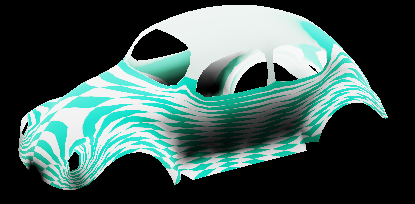
\includegraphics[width=3cm,height=2.5cm]{Beetle Uni.png}} & \raisebox{-0.5\height}{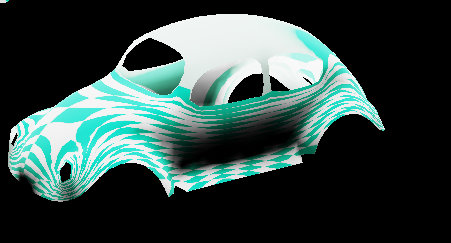
\includegraphics[width=3cm,height=2.5cm]{Beetle Cot.png}} & \raisebox{-0.5\height}{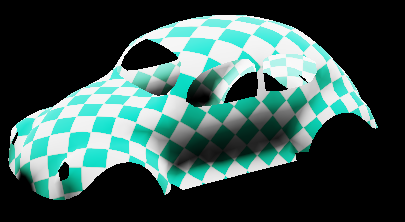
\includegraphics[width=3cm,height=2.5cm]{Beetle ASAP.png}} & \raisebox{-0.5\height}{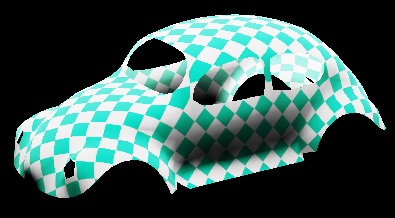
\includegraphics[width=3cm,height=2.5cm]{Beetle ARAP 10.png}} \\
	 		
	 		& & & & \\
	 		\hline
	 		\multirow{2}{*}{\textbf{Gar}} & \raisebox{-0.5\height}{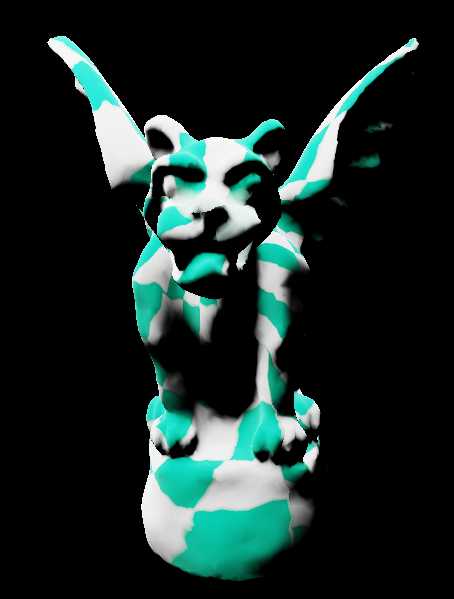
\includegraphics[width=3cm,height=2.5cm]{Gar Uni.png}} & \raisebox{-0.5\height}{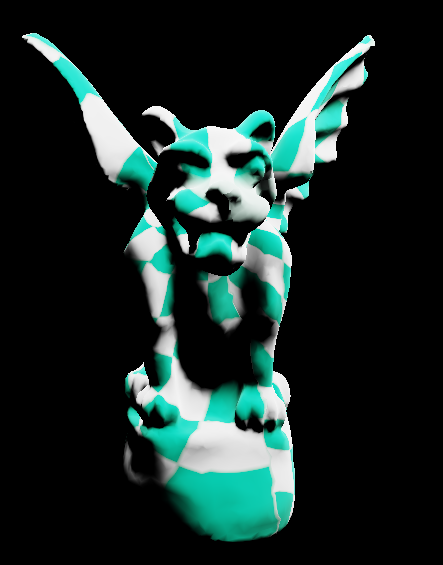
\includegraphics[width=3cm,height=2.5cm]{Gar Cot.png}} & \raisebox{-0.5\height}{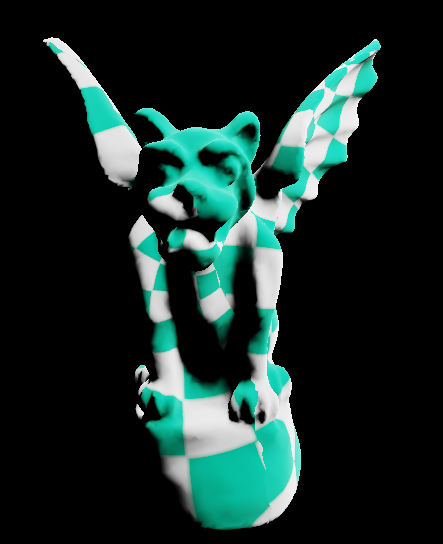
\includegraphics[width=3cm,height=2.5cm]{Gar ASAP.png}} & \raisebox{-0.5\height}{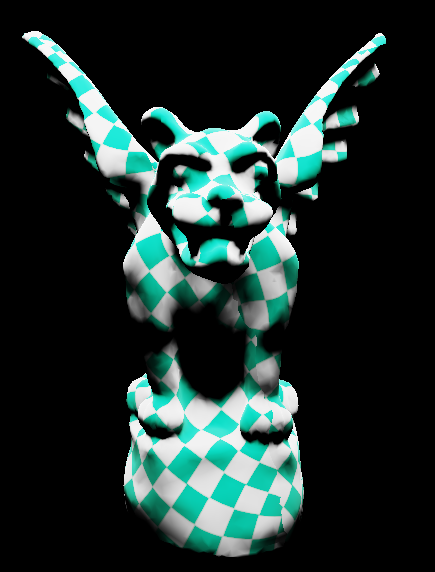
\includegraphics[width=3cm,height=2.5cm]{Gar ARAR 10.png}} \\
	 		
	 		
	 		
	 		& & & & \\
	 		\hline
	 		\multirow{2}{*}{\textbf{Isis}} & \raisebox{-0.5\height}{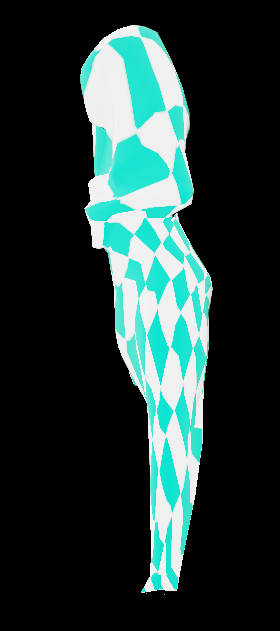
\includegraphics[width=3cm,height=3.5cm]{Isis Uni.png}} & \raisebox{-0.5\height}{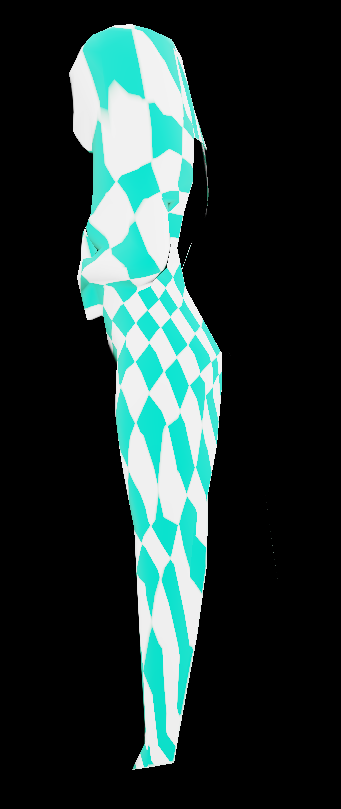
\includegraphics[width=3cm,height=3.5cm]{Isis Cot.png}} & \raisebox{-0.5\height}{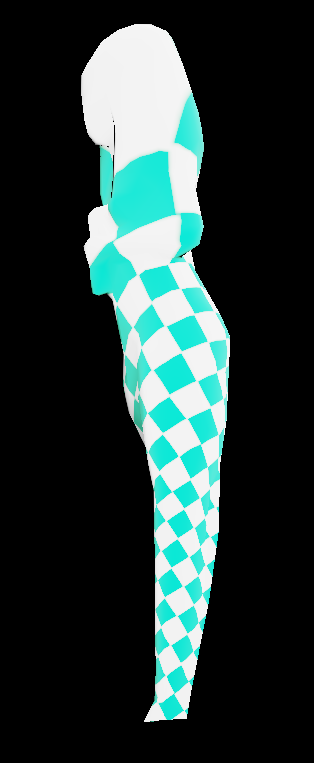
\includegraphics[width=3cm,height=3.5cm]{Isis ASAP.png}} & \raisebox{-0.5\height}{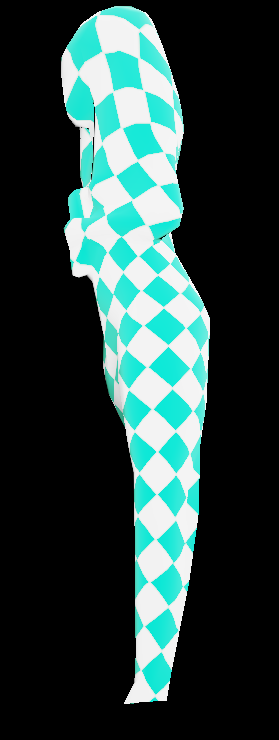
\includegraphics[width=3cm,height=3.5cm]{Isis ARAP.png}} \\
	 		
	 		& & & & \\
	 		\hline
	 		\multirow{2}{*}{\textbf{Cow}} & \raisebox{-0.5\height}{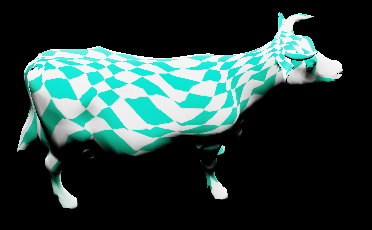
\includegraphics[width=3cm,height=2.5cm]{Cow Uni.png}} & \raisebox{-0.5\height}{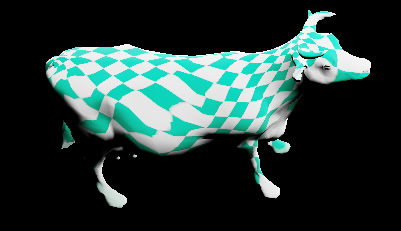
\includegraphics[width=3cm,height=2.5cm]{Cow Cot.png}} & \raisebox{-0.5\height}{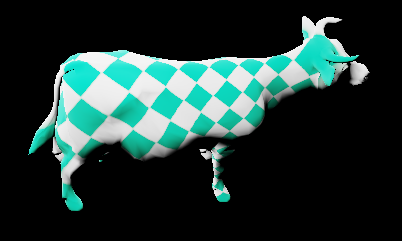
\includegraphics[width=3cm,height=2.5cm]{Cow ASAP.png}} & \raisebox{-0.5\height}{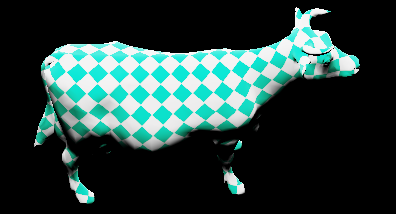
\includegraphics[width=3cm,height=2.5cm]{Cow ARAP 10.png}} \\
	 		
	 		
	 	
	 		& & & & \\
	 		\hline
	 	\end{tabular}
	 	\caption{主要结果}
	 \end{table}
 

   	 \begin{table}[htbp]
   	\centering
   	\setlength{\fboxsep}{0pt} % 重置图像的内边距
   	\begin{tabular}{|c|c|c|c|c|}
   		\hline
   		\diagbox[width=3cm]{\textbf{测试例子}}{\textbf{迭代次数}} & \textbf{1次} & \textbf{2次} & \textbf{5次} & \textbf{10次} \\
   		\hline
   		\multirow{2}{*}{\textbf{Beetle}} & \raisebox{-0.5\height}{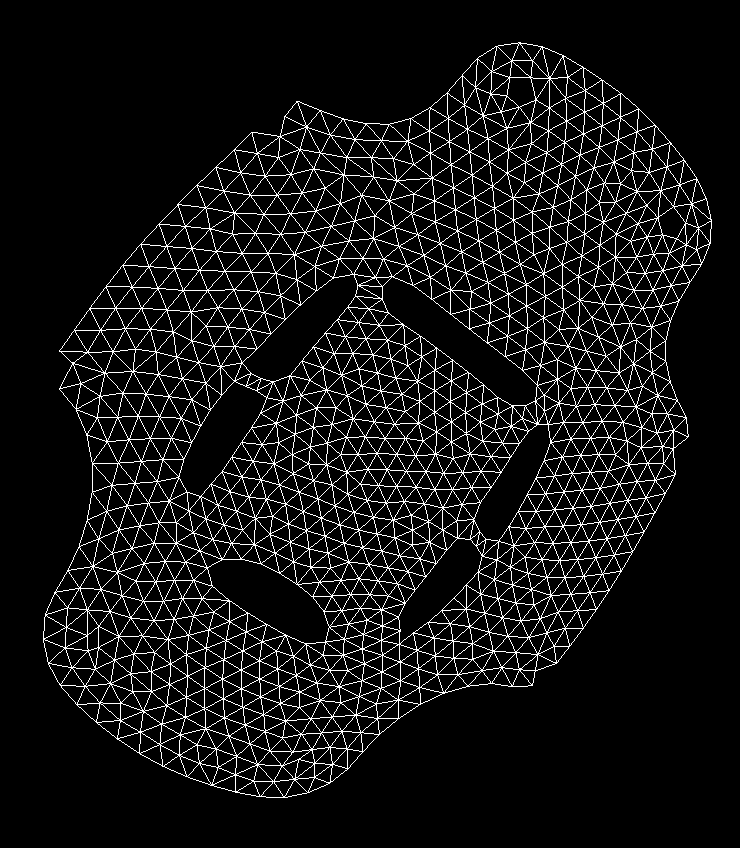
\includegraphics[width=3cm,height=2.5cm]{Beetle ARAP 1 wang.png}} & \raisebox{-0.5\height}{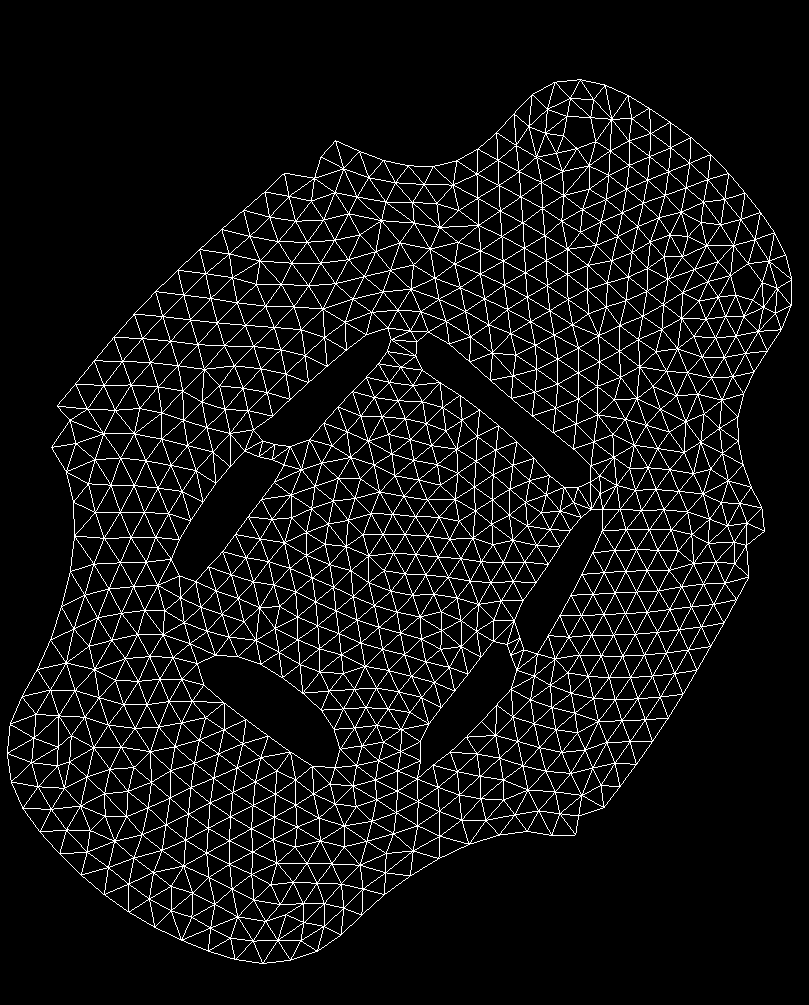
\includegraphics[width=3cm,height=2.5cm]{Beetle ARAP 5 wang.png}} & \raisebox{-0.5\height}{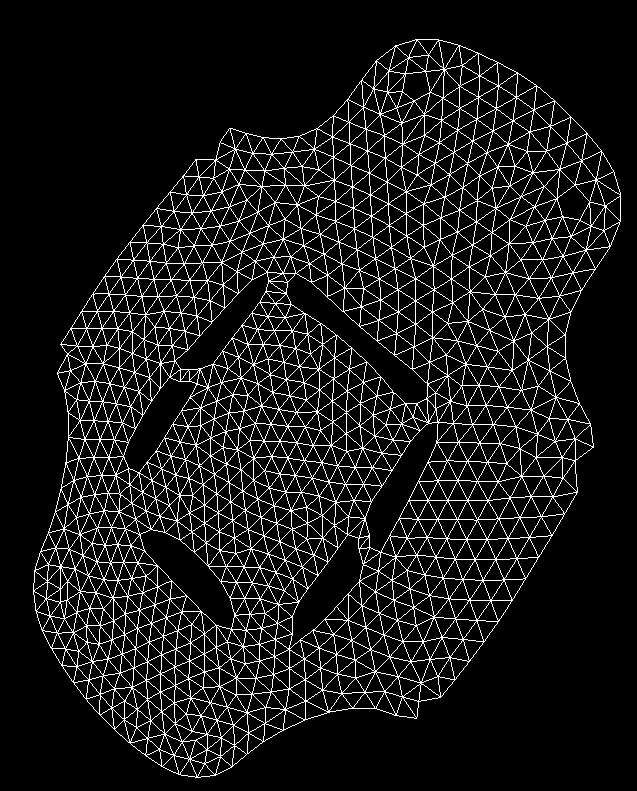
\includegraphics[width=3cm,height=2.5cm]{Beetle ARAP 10 wang.png}} & \raisebox{-0.5\height}{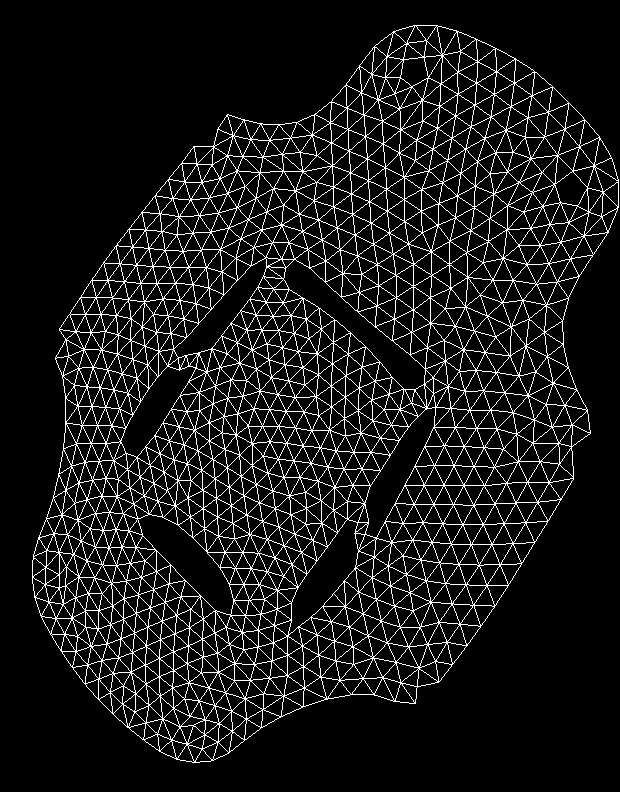
\includegraphics[width=3cm,height=2.5cm]{Beetle ARAP 20 wang.png}} \\
   		
   		& & & & \\
   		\hline
   		\multirow{2}{*}{\textbf{Balls}} & \raisebox{-0.5\height}{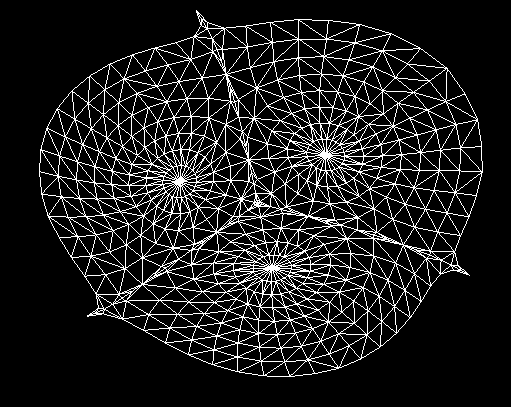
\includegraphics[width=3cm,height=2.5cm]{Balls wang 1.png}} & \raisebox{-0.5\height}{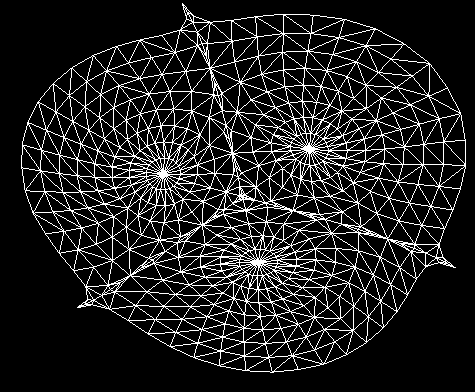
\includegraphics[width=3cm,height=2.5cm]{Balls wang 2.png}} & \raisebox{-0.5\height}{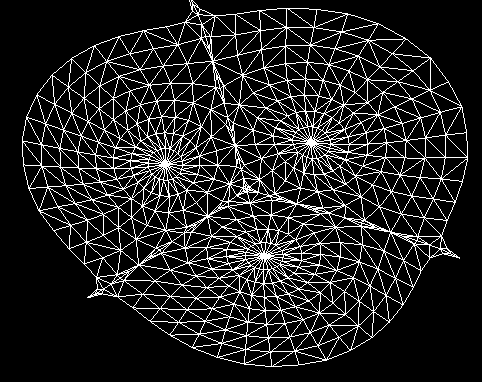
\includegraphics[width=3cm,height=2.5cm]{Balls wang 5.png}} & \raisebox{-0.5\height}{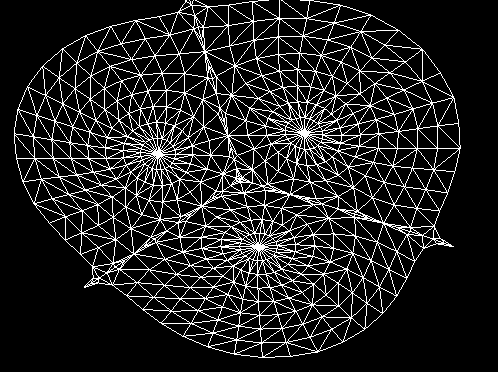
\includegraphics[width=3cm,height=2.5cm]{Balls wang 10.png}} \\
   		
   		
   		
   		& & & & \\
   		\hline
   	\multirow{2}{*}{\textbf{Cow}} & \raisebox{-0.5\height}{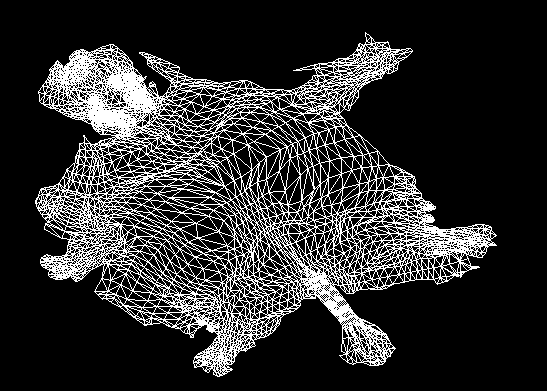
\includegraphics[width=3cm,height=2.5cm]{Cow wang 1.png}} & \raisebox{-0.5\height}{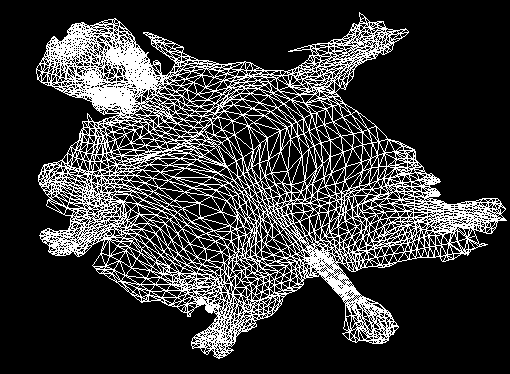
\includegraphics[width=3cm,height=2.5cm]{Cow wang 2.png}} & \raisebox{-0.5\height}{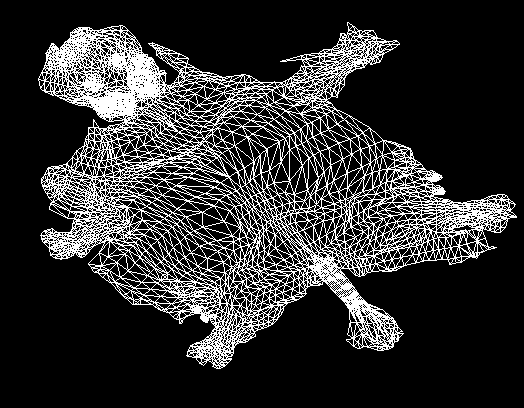
\includegraphics[width=3cm,height=2.5cm]{Cow wang 5.png}} & \raisebox{-0.5\height}{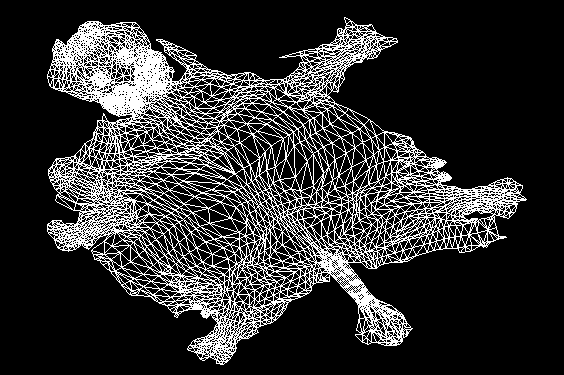
\includegraphics[width=3cm,height=2.5cm]{Cow wang 10.png}} \\
   		
   
   		& & & & \\
   		\hline
   	\end{tabular}
   	\caption{ARAP不同迭代次数对结果的影响}
   \end{table}
	
	
	\section{总结与讨论}
	

	 
	 从测试结果可以看出迭代次数会略有影响,但影响不大,基本上肉眼难以察觉。一般只需迭代1至2次就能得到很好的结果,迭代次数过多反而浪费性能,不划算。
	 
	 	 从图中可以看出ASAP和ARAP两种算法都是优于HW4的参数化方法的。它们生成的网格更均匀、光滑一些。而ARAP更是优于ASAP的,生成的网格基本上十分均匀,没有不规则的地方。综上,ARAP的性能是十分优良的。
	 
	
	
	
\end{document}